\section{Implementation Plan}
In this section we explain the order i which we plan to implement the subcomponents of the Travlendar+ system.
The main criteria we've adopted is to implement first a core of functionalities that we consider to be essential for engaging an initial user base, then we will proceed to insert new and nice-to-have features but that are not mandatory in a first release.
These are the main steps of the implementations we want to follow to reach Travlendar+ full operativity on\begin{large}
\textbf{server side}:
\end{large}
\begin{enumerate}
\item CalendarManager (AuthenticationManager, PathManager, EventManager, ScheduleManager, but not PreferenceManager), PersistenceManager and AuthenticationManager are the core of our system and so they are the first to be implemented among with their sub components. In particular in this phase the user will not be able to edit his travels but he can only visualize the proposed ones;
\item PreferenceManager will be inserted in a second release in order to filter the user paths and doing so will be added functionalities in order to allow the user to edit and choose the travels he prefer from the feasible ones proposed to him;
\item ComplicationManager will be added together with the NotificationManager in order to discover if a users travel is no more feasible and notify him.
\item TripManager will be the last module to be implemented, allowing the user to arrange his trips.
\end{enumerate}
Of course at each implementation phase some data structures are to be added in the database (through the PersistenceManager) to proper support the new functionalities.

These are the main steps of the implementations we want to follow to reach Travlendar+ full operativity on\begin{large}
\textbf{client side}:
\end{large}
\begin{enumerate}
\item Android App is to be developed first, proper updated will be performed when a new functionality is added on server-side, but the first application version is to be released together with the Application-server core functionality release.
\item IOS App will be developed in a second phase: when the Android application is completed (first release)the workforce dedicated to his development will be moved on this task but Android App's support will be taken care of nonetheless;
\item When both IOS and Android applications are released we will proceed to develop the web server that will allow the users to use Travlendar+ in any web browser.
\end{enumerate}

\section{Integration Entry Criteria}
Before starting the integration testing phase there are a number of conditions that have to be met:
\begin{itemize}
\item \textbf{Documents:} this document (DD) and RASD have to be completed;
\item \textbf{Proper Documentation:} Every method and class, before being tested must be provided with proper documentation and/or comments in order to ease the testing process and also make easier the reuse of the classes and their methods.
\item \textbf{Code Inspection and Analysis:} At least one method, either code inspection or automated or automated data flow analysis, have to be performed on the modules and classes before we proceed to the integration and test phase that involve them.
\item \textbf{Starting Condition:} The integration process can start only if the component involved offers at least 75\% of their functionalities to-be-implemented, this means that this phase can start in parallel with the completion of that component, and not that the testing phase can end with some functionalities still to be implemented; 
\item \textbf{Unit tests:} Before starting the integration of one component, it must be tested through proper unity tests, in order to guaranteed a correct behavior of his internal mechanisms.
\end{itemize}
\section{Elements to be integrated}
Basically all the system components, specified in section \ref{sect:Component view} need to be integrated together; here we specify in detail all the integration that need to be performed.
On Application Server side:
\begin{itemize}
	\item ScheduleManager, EventManager and PathManager needs to be integrated together;
	\item PreferenceManager needs to be integrated with PathManager (nb.doing do the entire CalendarManager subsystem will be integrated);
	\item TripManager needs to be integrated with ComplicationManager;
	\item ComplicationManager needs to be integrated with both NotificationManager and TripManager;
	\item PersistenceManager needs to be integrated with our DBMS;
	\item All the components that rely on RESTful APIs to implement the communication with the clients need to be integrated and tested;
	\item basically all the application server components rely on PersistenceManager and therefore they need to be integrated with it, the same consideration is valid for the AuthenticationManager (except for the NotificationManager that does not interact with it).
\end{itemize}
On client side (App Mobile):
\begin{itemize}
	\item DBManager needs to be integrated with the LocalDatabase;
	\item ApplicationController, GUIManager and DBManager needs to be integrated together;
\end{itemize}
On web server side WebController and JavaServerPages needs to be integrated together.
All the interactions that single components have with external services APIs have to be tested and their correctness have to be guaranteed before integrate and test phase involving those components begins.

\section{Integration Testing Strategy}
The integration testing strategy we will adopt will be defined by a mix of two strategies and according to the  implementation plan:
The first strategy we are going to use is based on a \textbf{bottom-up approach}. This choice will allow us to start from the less-dependent components and then climb the "uses" hierarchy, through the use of proper drivers. The bottom-up approach will enable us to follow the implementation plan, that follow the same approach. doing so we will improve the efficiency and the parallelism of the development process. \newline
The bottom-up strategy will be mixed with a \textbf{critical-module-first approach}, in order to start the integration and testing of the most critical module of our system, CalendarManager. We've considered also this second strategy in order to avoid issues related to core components of our system and threats to the correct behavior of our system, especially to guarantee the absence of failures or bugs that could prevent the users to correctly take advantage of our platform and its functionalities.

\section{Sequence of Components integration}
The following subsections aim to describe the order in which Travlendar+ will have to be integrated and tested. We will use as notation an arrow going from component A to component B means that component A is necessary to component B and so it must have been already implemented before performing the integration.

\subsection{Software integration Sequence}
Since our system rely on some external systems and interact with theirs external interfaces (APIs) we will assume that those system are already proper tested.
\subsubsection{PersistenceManager}
\begin{figure}[H]
	\begin{center}
		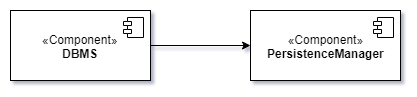
\includegraphics[scale=0.7]{implementation_and_testing/persistence.png}
	\end{center}
	\caption{I\&T-PersistenceManager}
\end{figure}
with db

\subsubsection{AuthenticationManager}
\begin{figure}[H]
	\begin{center}
		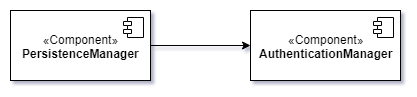
\includegraphics[scale=0.7]{implementation_and_testing/authentication.png}
	\end{center}
	\caption{I\&T-AuthenticationManager}
\end{figure}
with PersistenceManager

\subsubsection{CalendarManager}
\begin{figure}[H]
	\begin{center}
		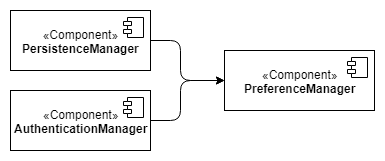
\includegraphics[scale=0.7]{implementation_and_testing/calendar_manager/preference.png}
	\end{center}
	\caption{I\&T-PreferenceManager}
\end{figure}

\begin{figure}[H]
	\begin{center}
		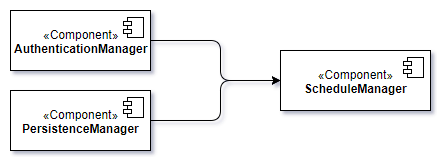
\includegraphics[scale=0.7]{implementation_and_testing/calendar_manager/schedule.png}
	\end{center}
	\caption{I\&T-ScheduleManager}
\end{figure}

\begin{figure}[H]
	\begin{center}
		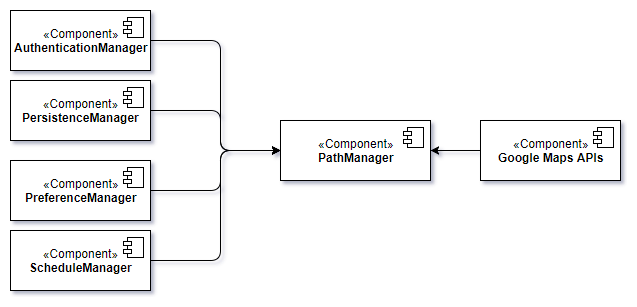
\includegraphics[scale=0.7]{implementation_and_testing/calendar_manager/path.png}
	\end{center}
	\caption{I\&T-PathManager}
\end{figure}

\begin{figure}[H]
	\begin{center}
		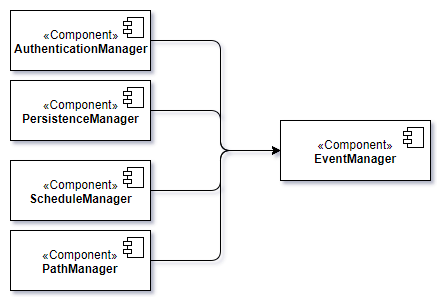
\includegraphics[scale=0.7]{implementation_and_testing/calendar_manager/event.png}
	\end{center}
	\caption{I\&T-EventManager}
\end{figure}
all with PersistenceManager (man mano)
path with google maps
schedule-path-event-preference
all with Authentication

\subsubsection{TripManager}
\begin{figure}[H]
	\begin{center}
		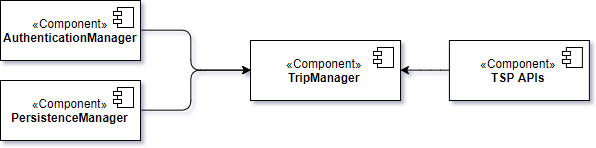
\includegraphics[scale=0.7]{implementation_and_testing/trip.png}
	\end{center}
	\caption{I\&T-TripManager}
\end{figure}
PersistenceManager/TSP api

\subsubsection{NotificationManager}
\begin{figure}[H]
	\begin{center}
		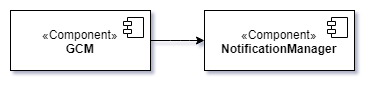
\includegraphics[scale=0.7]{implementation_and_testing/notification.png}
	\end{center}
	\caption{I\&T-NotificationManager}
\end{figure}
GCM

\subsubsection{ComplicationManager}
\begin{figure}[H]
	\begin{center}
		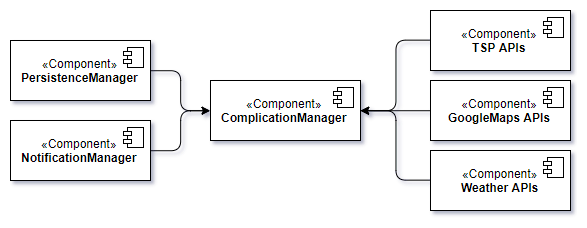
\includegraphics[scale=0.7]{implementation_and_testing/complication.png}
	\end{center}
	\caption{I\&T-ComplicationManager}
\end{figure}
google maps/TSP/Weather/NotificationManager

\subsubsection{WebServer}
\begin{figure}[H]
	\begin{center}
		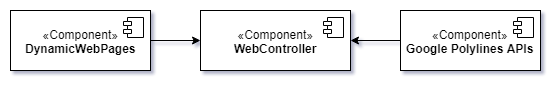
\includegraphics[scale=0.7]{implementation_and_testing/web.png}
	\end{center}
	\caption{I\&T-WebServer}
\end{figure}
web with JSP +polylines

\subsubsection{AppMobile}
\begin{figure}[H]
	\begin{center}
		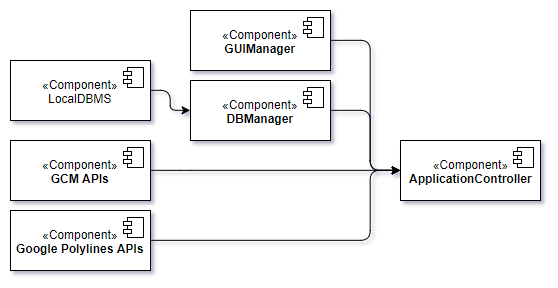
\includegraphics[scale=0.7]{implementation_and_testing/app.png}
	\end{center}
	\caption{I\&T-AppMobile}
\end{figure}
local db/db manager
db manager/gui with application controller
GCM/Google polylines

\subsection{Subsystems integration Sequence}
google pol